\section{Modellierung}
\subsection{Systembeschreibung}
\begin{figure}[H]
	\centering
	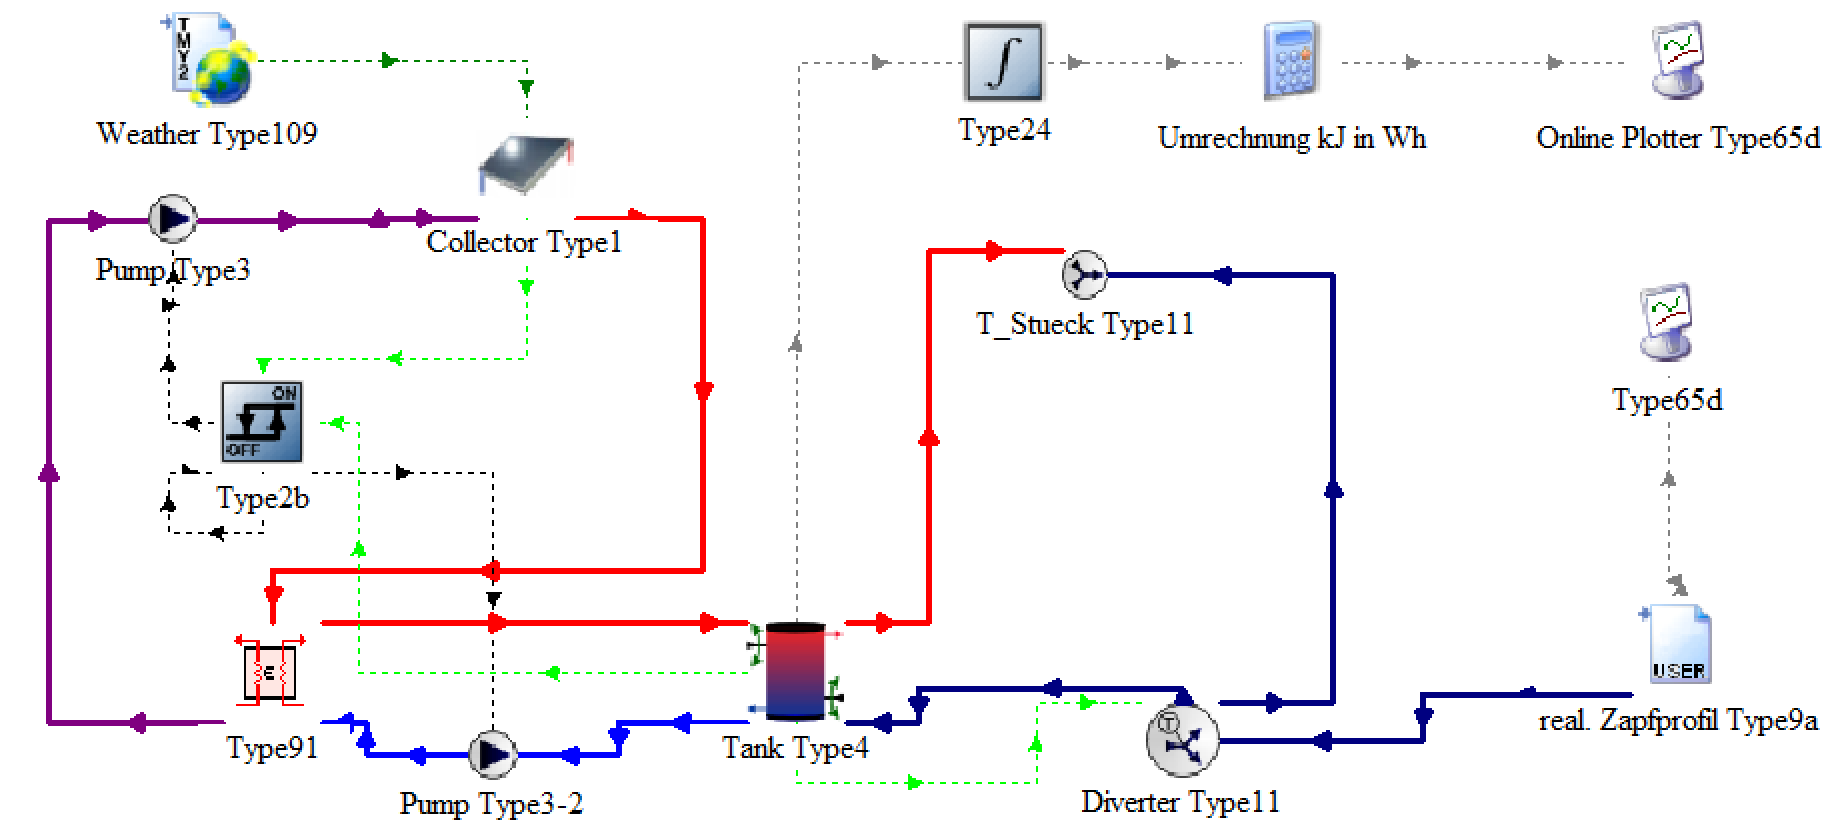
\includegraphics[width=0.8\textwidth]{../DATA/std_deck.png}
	\caption[Grundsystem]{Grundsystem}
	\label{fig:std_deck}
\end{figure}

Das System basiert auf einem Speicher mit integrierter Nachheizung sowie einem angeschlossenen Kollektor, welcher mit Wetterdaten gespeist wird. Der Massenstrom des Kollektorkreislaufes wird 

\subsection{Systemanpassung: Verluste}


\subsection{Systemauslegung}
Anhand der Wetterdaten von Stuttgart soll eine solare Deckung von 60\,\% für das vorliegende Zapfprofil erzielt werden.

\begin{equation}
	\label{eq:fsolin}
	f_{sol,in} = \frac{Q_{sol}}{Q_{sol}+Q_{aux}}
\end{equation}

\begin{equation}
	\label{eq:}
	f_{sol,out} = \frac{Q_{sol}-Q_{verl,Sp}}{Q_{TWW+RH}+Q_{Zirk}}
\end{equation}
\section{Parametervariation}
\subsection{Kaltwasser- und Umgebungstemperatur des Speichers}
\begin{center}
	\begin{tabular}{l|c|c}
		\label{tab:}
		
		\textbf{} & \textbf{} & \textbf{}\\
		\hline
		&  & \\
		&  & \\
	\end{tabular}
\end{center}


\subsection{Rohrlänge und -dämmung}

\section{Optimierung der Kollektorparameter}
